\section{LL-Eigenschaften}
Seite 166 im Script stehen die Eigenschaften \\
Wie andere Grammatik transformiert findet man im Script auf Seite 169
Eine Grammatik kann nicht die LL-Eigenschaften erfüllen wenn sie linksrekursion bzw. linksgleiche Produktionen enthält (Was sind Produktionen?)
Allgemeine Elimination von linksrekursion auf Seite 171 im Script
\begin{align*}
    A::= A \alpha \\
    \Longrightarrow \\
    A::= \beta A' \\
    A'::=\alpha A' | \epsilon
\end{align*}

Definition (Linksfaktorisierung). Problem $FIRST(..FOLLOW(..))$ nicht disjunkt:
\begin{align*}
  A::=\alpha \beta_1  |  \alpha \beta_2 \\
  \Longrightarrow\\
  A::= \alpha A'\\
  A'::= \beta_1  |  \beta_2
\end{align*}
$FF_1 = FIRST(T E' FOLLOW(E))={i*}$ das in den geschweiften Klammern ist das $First(T)$ wenn $\epsilon$ nicht in der First-Menge ist. 
Falls doch ist es das $First$ vom nächssten nicht Terminal. 
Falls alle ein $\epsilon$ in ihrer First\_Menge haben ist es das $Follow(E')$.\\
\\

\subsection{LL-Bedingungen \label{ref}}
Die Grammatik erfüllt die LL-Bedingungen wenn die gleichen Follows in den First-Follow-Mengen einen unterschiedlichen Inhalt haben.
\begin{align*}
  FF_1 = FIRST(T E' FOLLOW(E))={i*}\\
  FF_2 = FIRST(\epsilon FOLLOW(E))={\#}
\end{align*}



\subsection{LL-Automaten}
Seite 177 findet man die LL-Automaten \\
\begin{itemize}
  \item Der LL-Automat erzeugt eine Linksableitung des Eingabewortes
  \item Erfüllt $G$ die LL-Bedingungen, dann kann ein deterministischer Automat konstruiert werden.
\end{itemize}

\begin{enumerate}
  \item Transfomieren Sie die Grammatik, so dass die Grammatik die LL(1) Bedingung erfüllt
  \item Erstellen Sie den nichtdeterministischen LL(1)-Automaten für diese Grammatik
  \item Erstellen Sie hieraus den deterministischen LL(1)-Automaten\\ (nun ja er ist nicht ganz deterministisch, da die Produktionen eines Nichtterminals die LL(1) Bedingung nicht erfüllt, erstellen Sie den Automaten trotzdem!)\\
  Markieren Sie die nichtdeterministischen Automatenregeln.
  \item Akzeptieren Sie mit diesem Automaten das "Programm" i + i[i+i]
\end{enumerate}
Beispiel Aufgabe auf Seite 179 im Script\\
\begin{itemize}
  \item Grammatik linksrekursion rausbekommen
  \item First-Follow-Menge berechnen 
  \item LL1 Eigenschaften herausfinden
  \item Automat
  \item Automat mit First-Follow
\end{itemize}
Die Regel schreib man einfach umgekehrt zur Grammatik.
\begin{align*}
  E' ::= +TE'\\
  E'qt\longrightarrow E'T+
\end{align*}


\section{LR-Automaten}

\begin{center}
  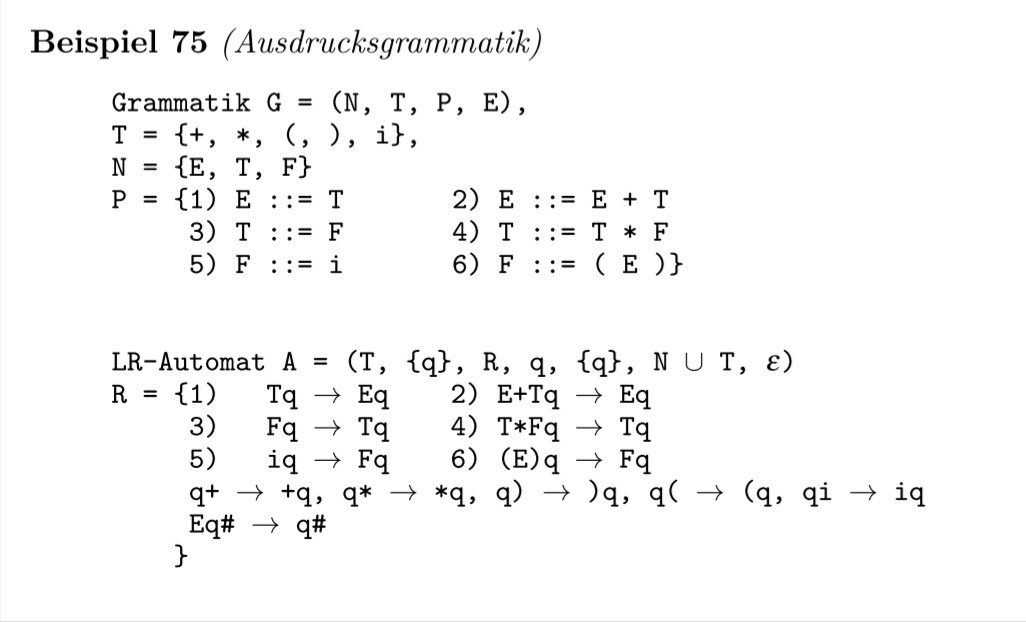
\includegraphics[height=7cm]{image/Screenshot 2022-12-10 170319.jpg}
\end{center}
\begin{center}
  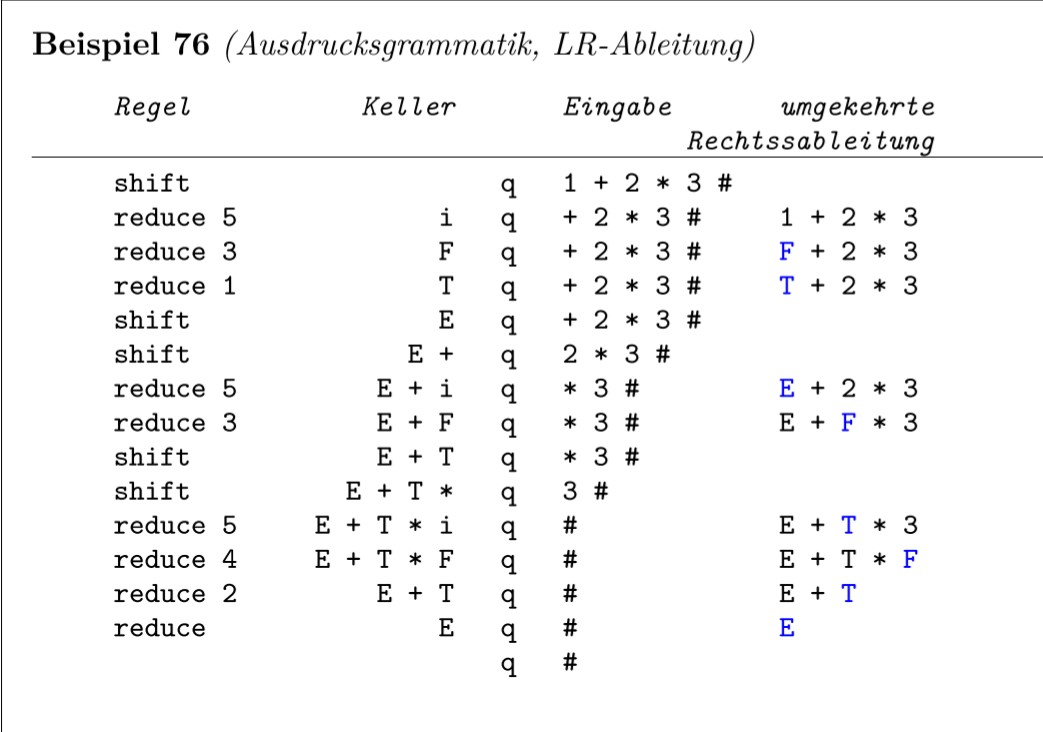
\includegraphics[height=7.5cm]{image/Screenshot 2022-12-10 170336.jpg}
\end{center}
\subsection{Konflikte}
\subsubsection*{Shift/Reduce}
Mehrdeutigkeit wird unterbunden in dem bevorzugt gesschiftet wird. $\Longrightarrow$ Lösung Dangeling-Else Problem.
Nicht immer shiften Operatorvorrang (Skript Seite 198f)
\subsubsection*{Reduce/Reduce}
Macht es einen Unterschied?\\
Wenn nicht eine Regel wegschmeisen 
